\section{Zielsetzung}
Das Ziel des vorliegenden Versuchs ist es sich anhand von Monte-Carlo-Simulationsdaten mit der Neutrinoselektion am IceCube-Experiment vertraut zu machen. Zum Durchführen der Seperation werden verschiedene Methoden des Maschinellen Lernens verwendet.
\section{Theorie}
Die aktuellen Erkenntnisse in der Astrophysik basierten darauf, dass im 20.Jahrhundert die optische Astronomie auf andere Wellenlängenbereiche erweitert werden konnte. Heutzutage werden neben dem optische Bereich, auch Radio-, Röntgen-, Infrarot-, und Ultraviolettastronomie entwickelt.\\
Entscheidend ist zudem die durch Victor Heß im Jahre 1912 entdeckte Höhenstrahlung. Sie war bis in die 1950er Jahre die einzige Quelle hochenergetischer Teilchen. Ihre Entdeckung zeigte, dass die Erde bzw. die Atmosphäre neben Photonen auch von anderen Teilchen getroffen wird. Beim Auftreffen der geladenen kosmischen Strahlung ,der sogenannten Primärteilchen, kommt es zur Wechselwirkung mit der Atmosphäre, sodass Teilchenkaskaden aus Sekundärteilchen entstehen. Diese lassen sich über verschiedenen Methoden abhängig von ihren Teilcheneigenschaften nachweisen. Die geladenen kosmische Strahlung setzt sich neben Protonen aus Helium und anderen schweren Kernen zusammen, wobei die genau Zusammensetzung von dem Energiebereich abhängt. Dieses Spektrum wird durch ein Potenzgesetz beschrieben:
\begin{align}
	\frac{\text{d}\Phi}{\text{d}E} = \Phi_{0} \cdot E^{\gamma}
\end{align}
Der spektrale Index $\gamma$ liegt für die geladene Höhenstrahlung bei $\gamma \approx -2.7$. Dies liegt vor allem daran, dass geladene Materie auf ihrem Weg zur Erde durch galaktische und extragalaktische Magnetfelder abgelenkt werden. Dies verhindert eine Richtungsrekonstruktion, sodass auch ihre Quellen bisher unbekannt sind.
\subsection{Klassifizierung von Leptonen}
Bei IceCube werden Leptonen, hauptsächlich Myonen und Neutrinos untersucht. Diese können sowohl aus der Höhenstrahlung als auch astrophysikalischen Quellen stammen und unterscheiden sich durch ihre Energieverteilung und damit dem spektralen Index. \\
Die Atmosphärischen Myonen und Neutrinos werden außerdem in konventionelle und prompte unterschieden. Die Konventionellen entstehen, wenn bei der Wechselwirkung der geladenen kosmischen Strahlung Pionen oder Kaonen erzeugt werden. Durch ihre teilweise lange Lebensdauer verlieren diese Mesonen Energie, bevor sie in die konventionellen Myonen bzw. Neutrinos zerfallen. Daher gilt für das Spektrum der konventionellen Myonen und Neutrinos $\propto E^{-3.7}$.\\
Bei der Wechselwirkung der geladenen kosmischen Strahlung mit der Atmosphäre können jedoch auch kurzlebige, schwere Hadronen, wie $D$-Mesonen oder $\Lambda_{c}$-Baryonen entstehen. Diese zerfallen ohne nennenswerte Energieverluste weiter in die promten Myonen und Neutrinos. Daher ist deren Spektrum  $\propto E^{-2.7}$ und somit direkt vererbt von der geladenen kosmischen Strahlung.\\
Es wird davon ausgegangen, dass astrophysikalische Quellen, die Hadronen beschleunigen auch Neutrinos und hochenergetische Photonen emittieren. Da sie ungeladen sind, werden sie nicht durch äußere Magnetfelder abgelenkt und liefern somit Informationen über ihren Ursprung. Der Vorteil von Neutrinos im Gegensatz zu Photonen ist, dass sie durch ihren sehr kleinen Wirkungsquerschnitt ebenfalls Staubwolken und optisch dichte Medien durchdringen können und somit Informationen über das optisch dichtere Innere eines astrophysikalischen Objektes liefern. Unter Annahme von Stoßbeschleunigung nach Fermi \cite{PhysRev.75.1169}, besitzt der astrophysikalische Neutrinofluss einen spektralen Index von  $\propto E^{-2}$.\\
\subsection{Das IceCube-Experiment}
Das IceCube-Experiment wird zur Detektion von hochenergetischen Neutrinos und Myonen genutzt. Es befindet sich am geographischen Südpol in einer Tiefe von $1450-\SI{2450}{\meter}$ unter der Oberfläche in einer klaren Eisschicht. Insgesamt setzt sich der Detektor aus den drei Komponenten Ice-Top \cite{3246225}, In-Ice-Array \cite{ACHTERBERG2006155} und DeepCore \cite{2143409} zusammen. Eine schmatische Darstellung des Detektors befindet sich in Abbildung \ref{fig:Ice}.
\begin{figure}
  \centering
  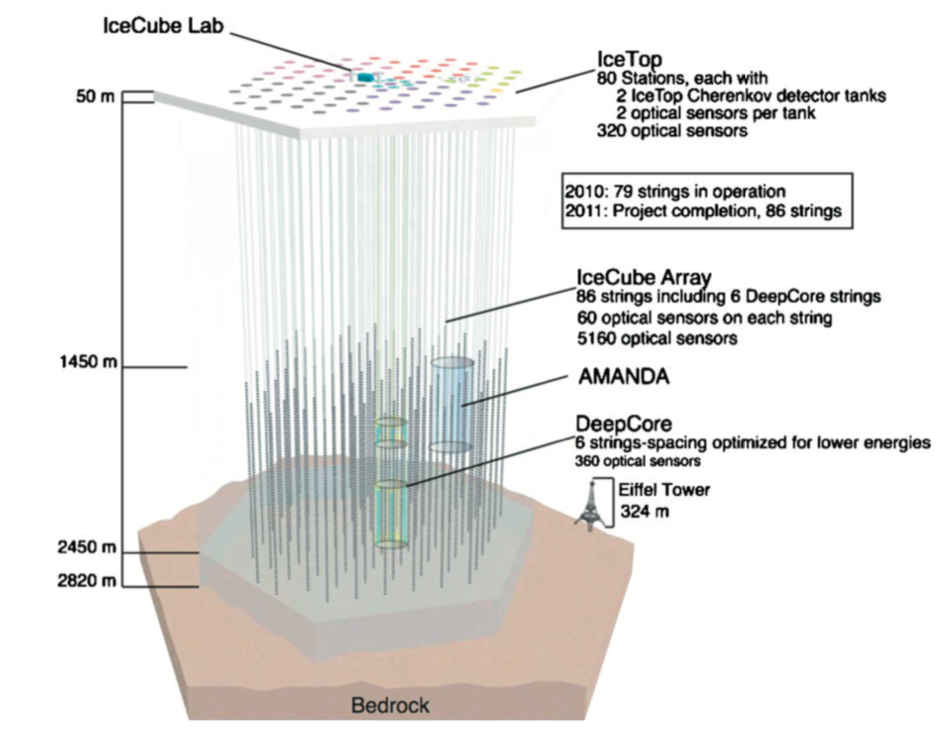
\includegraphics[width=0.5\textwidth]{graphics/IceCube.png}
  \caption{Schematische Darstellung des IceCube-Detektors mit seinen drei Komponenten Ice-Top, In-Ice-Array und DeepCore.\cite{IceCube}}
  \label{fig:Ice}
\end{figure}
Zu Teilchendetektion wird sich dabei das Prinzip von Tscherenkov-Licht zu nutze gemacht. Dieses wird emittiert, wenn sich ein hochenergetisches, geladenes Teilchen überlichtschnell im Medium bewegt. Die Lichtgeschwindigkeit im Medium ist $c=\frac{c_{0}}{n}$, wobei $n$ dem Brechungsindex des Mediums entspricht und $c_{0}$ der Vakuumlichtgeschwindigkeit. Dieses Tscherenkov-Licht kann mit 5160 Photoelektronenvervielfachern aufgenommen werden, die auf insgesamt 86 Kabel verteilt sind.\\
Diese bilden grundsätzlich das In-Ice-Array, das eine Energieschwelle von $\SI{100}{\giga\electronvolt}$ besitzt. Der DeepCore besteht aus 7 Kabeln, die dichter zusammenliegen und eine höhere Photomultiplierdichte besitzen. Daher bildet er die Niederenergieerweiterung des Detektors und hat eine Energieschwelle von bereits $\SI{10}{\giga\electronvolt}$.\\
Das IceTop ist ein Luftschauer-Experiment aus lichtdichten Eistanks. Es dient mithilfe von Tscherenkov-Licht sowohl zur Untersuchung von kosmischer Strahlung als auch als Veto für das In-Ice-Array. So können zum Beispiel atmosphärische Teilchen von Neutrinos, die die Erde durchquert haben, unterschieden werden.\\
